\chapter{Implementation and Results}

This chapter focuses on comparing the performance between \acrshort{mcmc} and \acrshort{vi} methods for performing inference in a \acrshort{pgm}. Each method have their strengths and weaknesses for different types of problems. As a compromise, this chapter will focus on comparing the performance of a fictitious model in order to discuss a concrete example and to show how \acrshort{mcmc} and \acrshort{vi} can be used in practice.  

\section{The model}
As the context of this paper is intention inference for autonomous ferries, it seems fit that a similar example is used. A simple intention model is therefore proposed as an example, which relates steering angle to an intention through a mixture model. 

The angle $\theta_t$ is defined to be the angle between the obstacles current course and the predicted course given the obstacles final destination. The vessels are required to report their final destination, but in some cases there may be user-errors where invalid destinations are transmitted to nearby vessels. If the obstacles report the final destination is correctly, $D_t=0$, the angle should be closely related to the obstacles intention and can be generated from a Gaussian selected by the intention $I_t$ (i.e. a mixture of Gaussian's weighted by the intention probabilities). If the obstacle report an incorrect destination, $D=1$, the angle $\theta_t$ is independent of intention as the obstacle may he headed in a completely different direction.

This example model is intentionally not identifiable when observing only the angles $\theta_t$. This example will show how the choice of priors affect the learning process, especially when parameters are not identifiable. Through the use of informative priors the model should still be able to learn what it can from available data.   

Whether or not the final destination is valid is modelled using a Bernoulli variable $D_t$ which takes the value $1$ if the destinations is \textbf{invalid}. A Beta distribution is used to model the prior probability $p_D$ of $D=1$, i.e. the destination being invalid.  

\begin{description}
    \item[Assumption 1] The angles $\{\theta_1, \theta_2, \dots, \theta_t\}$ are independent
    \item[Assumption 2] The ship has equal turning characteristics for port and starboard turns. The intention probabilities are from this assumed symmetrical about $\theta=0$. 
    \item[Assumption 3] Port and starboard turns are defined to be turns where $\theta \in (0, \pi)$ and $\theta \in (-\pi, 0)$ respectively.  
\end{description}

\begin{equation}
    p_D \sim \text{Beta}, \quad p_D \in (0, 1)
\end{equation}
\begin{equation}
    D_t \sim \text{Bernoulli}(p_D), \quad D_t \in \{0, 1\}
\end{equation}

The intention in a situation $I_t$ is modelled by a Categorical discrete variable where the possible realizations are shown in \cref{tbl:intentions}. The intention probabilities $\boldsymbol{\alpha}$ are distributed according to a Dirichlet distribution.

\begin{equation}
    \boldsymbol{\alpha} \sim \text{Dirichlet}, \quad \boldsymbol{\alpha} \in \{\alpha_0, \alpha_1, \alpha_2 \in (0, 1) \; | \; \sum_i \alpha_i = 1 \}
\end{equation}
\begin{equation}
    I_t \sim \text{Categorical}(\boldsymbol{\alpha}), \quad I_t \in \{0, 1, 2\}
\end{equation}

\begin{table}[h]
\centering
\begin{tabular}{|l|l|}
\hline
$I_t=0$ & The obstacle intends to keep its current course \\ \hline
$I_t=1$ & The obstacle intends a starboard turn           \\ \hline
$I_t=2$ & The obstacle intends a port-side turn            \\ \hline
\end{tabular}
\caption{Possible realizations of the intention $I_t$}
\label{tbl:intentions}
\end{table}


The mixture components for $\theta_t$ when $D_t=0$ are Gaussian Distributions. For $I=0$, the mean is zero with unknown variance. For $I \in \{1, 2\}$ the means are assumed to have equal absolute value, but opposite sign. The value for $\mu = \mu_2 = -\mu_1$ is unknown and distributed according to a Gaussian variable. The standard deviation is assumed equal for all intentions and is distributed according to an inverse Gamma distribution. In other words, the mixture components are assumed to have the same variance and they should be symmetrical around $\theta_t=0$.
Learning the mean $\mu$ from data allows the model to adapt to different types of ships. A small fishing vessel might rapidly change course (i.e. large $\theta_t$), while a large oil-tanker has limited ability to turn due to its size (i.e. smaller $\theta_t$). 
\begin{align}
    \mu_0 &= 0 &  \mu_{2} = - \mu_{1} = \mu &\sim \text{Gaussian} & \sigma &\sim \text{Inv-Gamma}
\end{align}
When $D=0$ and $I_t=i$, the angle is distributed according to
\begin{equation}\label{eq:theta_intention_mixture}
    p(\theta_t | D=0, I_t=i) = \mathcal{N}(\mu_i, \sigma^2), \quad \theta_t \in \mathcal{R}
\end{equation}

The marginal distribution of $\theta_t$ when $D_t=0$ becomes the Gaussian mixture model in \cref{eq:angle_gauss_mixture}.

\begin{align}\label{eq:angle_gauss_mixture}
\begin{split}
    p(\theta_t | \boldsymbol{\mu}, \sigma, D=0, \boldsymbol{\alpha}) &= \sum_{i=0}^2 \Pr\{I_t=i\}\mathcal{N}(\theta_t | \mu_i, \sigma^2) \\
    &=\Pr\{I_t=0 | \alpha_0\}\mathcal{N}(\theta_t | 0, \sigma^2)\\
    &\quad+\Pr\{I_t=1 | \alpha_1\}\mathcal{N}(\theta_t | -\mu, \sigma^2)\\
    &\quad+\Pr\{I_t=2 | \alpha_2\}\mathcal{N}(\theta_t | \mu, \sigma^2)
\end{split}
\end{align}

One issue with using a Guassian distribution for angle information is that it has support on $\mathcal{R}$, while the angles $\theta$ should ideally only have support on $(-\pi, \pi)$. In practice, this may not be a big issue as long as the probability mass is mostly kept within $(-\pi, \pi)$. Another solution could be to use a nonlinear transformation to clamp $\mathcal{R}$ to $(-\pi, \pi)$. There is however a possible issue with the mean $\mu$ as it is implicitly assumed to be positive, even if the the Gaussian distribution offer support on $\mathcal{R}$. As the angle distribution is assumed symmetrical around $theta=0$, it is possible to swap the portside and starboard turn intentions by swapping the sign of $\mu$. This will likely cause the posterior distribution to become bimodal, as the data is unable to distinguish between the two intentions.  

\cref{fig:intention_angle} shows the likelihood for different angles for the different intentions with fixed mean and variance. 

When the obstacles target destination is invalid, $D=1$, the angle $\theta$ is distributed according to a Uniform distribution over the range $(-\pi, \pi)$ to model how the angle contains no information about the obstacle in such a case. 

\begin{equation}\label{eq:angle_uniform}
    p(\theta_t | D=1) = \text{Uniform}(-\pi, \pi)
\end{equation}

The distribution for $\theta_t$ becomes a mixture between the Gaussian Mixture in \cref{eq:angle_gauss_mixture} and the uniform distribution in  \cref{eq:angle_uniform} as expressed in \cref{eq:angle_complete_mixture} by the law of total probability.

\begin{align}\label{eq:angle_complete_mixture}
\begin{split}
     p(\theta_t | \boldsymbol{\mu}, \sigma, p_D, \boldsymbol{\alpha})
     &= \sum_D \Pr\{D_t=d | p_D\} p(\theta_t | D_t=d, \mu, \sigma, \boldsymbol{\alpha})\\
     &= \Pr\{D_t = 0 | p_D\} \underbrace{p(\theta_t | \mu, \sigma, D_t=0, \boldsymbol{\alpha})}_{\text{\cref{eq:angle_gauss_mixture}}}\\
     &+ \Pr\{D_t=1 | p_D\}\underbrace{p(\theta_t | D_t=1)}_{\text{\cref{eq:angle_uniform}}}
\end{split}
\end{align}

For multiple data points $\boldsymbol{\theta}$, the


The data generating process for $\theta_t$ is shown in \cref{fig:example_pgm} then becomes:

\begin{enumerate}
    \item Draw priors $p_D$, $\boldsymbol{\alpha}$ 
    \item Draw priors $\mu$ and $\sigma$
    \item For all $t \in \{1, \dots, N \}$, draw $D_t$ and $I_t$ conditional on $p_D$ and $\boldsymbol{\alpha}$
    \item For all $t \in \{1, \dots, N\} $, if $D_t=1$, draw $\theta_t$ from Uniform distribution. If not, draw $\theta_t$ from $\mathcal{N}(\theta_t | \mu_i, \sigma)$ conditional on $\mu_i$ and $\sigma$. 
\end{enumerate}

\begin{figure}[h]
    \centering
    \begin{tikzpicture}
        % NODES
        \node[latent] (I) {$I$};
        \node[obs, below=of I] (theta) {$\theta$};
        \node[latent, above=of I] (alpha){$\boldsymbol{\alpha}$};
        
        % FACTORS
        \factor[below=of I] {theta-f}{left:Mix}{}{};
        \factor[above=of I]{I-f}{right:Cat}{}{};
        \factor[above=of alpha]{PI-f}{right:Dir}{}{};

        \node[latent, left= of I] (D) {$D$};
        \node[latent, above= of D] (p_D) {$p_D$};
        \node[latent, right= of theta-f, yshift=1cm] (mean) {$\mu$};
        \node[latent, right= of theta-f] (std) {$\sigma$};

        \factor[right=of mean]{mean-f}{above:$\mathcal{N}$}{}{};
        \factor[right=of std]{std-f}{above:$\text{Gam}^{-1}$}{}{};
        \factor[above=of D]{D-f}{left:Bern}{}{};
        \factor[above=of p_D]{p_D-f}{left:Beta}{}{};

        \node[const, above=of p_D] (pp_D) {$\bar{p_D}$};
        \node[const, right=of mean] (p_mean) {$\bar{\mu}$};
        \node[const, right=of std] (p_std) {$\bar{\sigma}$};
        \node[const, above=of alpha] (a) {$\bar{\boldsymbol{\alpha}}$};
        
        \factoredge {I, D, mean, std} {theta-f} {theta};
        \factoredge{alpha}{I-f}{I};
        \factoredge{a}{PI-f}{alpha};
        \factoredge{p_mean}{mean-f}{mean};
        \factoredge{p_std}{std-f}{std};
        \factoredge{pp_D}{p_D-f}{p_D};
        \factoredge{p_D}{D-f}{D};

        \plate {ship}{(I)(theta)(D)}{$t \in T$};
    \end{tikzpicture}
    \caption{\acrshort{pgm} describing the data-generating process using graphical notation. The rectangle is called a plate and express that the variables within are repeated once for each $t \in T$. The variables outside the plate are shared across all $t \in T$. The gray node for $\theta$ indicate that the variable is observed, while the rest are latent.}
    \label{fig:example_pgm}
\end{figure}



The resulting joint distribution  can then be factored into \cref{eq:example_joint}.

\begin{align}\label{eq:example_joint}
\begin{split}
    p(\boldsymbol{\theta}, \boldsymbol{\mu}, \sigma, p_D, \boldsymbol{\alpha}) =\underbrace{p(\boldsymbol{\alpha})}_{\text{Dirichlet}}\underbrace{p(p_D)}_{\text{Beta}}\underbrace{p(\mu)}_{\mathcal{N}} \underbrace{p(\sigma)}_{\text{Inv-Gamma}} \prod_t \underbrace{p(\theta_t | \mu, \sigma, p_D, \boldsymbol{\alpha})}_{\text{\cref{eq:angle_complete_mixture}}}
\end{split}
\end{align}

The unnormalized posterior distribution then becomes
\begin{align}\label{eq:example_unnormalized_posterior}
\begin{split}
    \tilde{p}(\mu, \sigma, p_D, \boldsymbol{\alpha}) =  p(\boldsymbol{\theta} = \mathcal{D}, \mu, \sigma, p_D, \boldsymbol{\alpha}) \propto p(\mu, \sigma, p_D, \boldsymbol{\alpha} | \boldsymbol{\theta}= \mathcal{D})
\end{split}
\end{align}


\begin{figure}
    \centering
    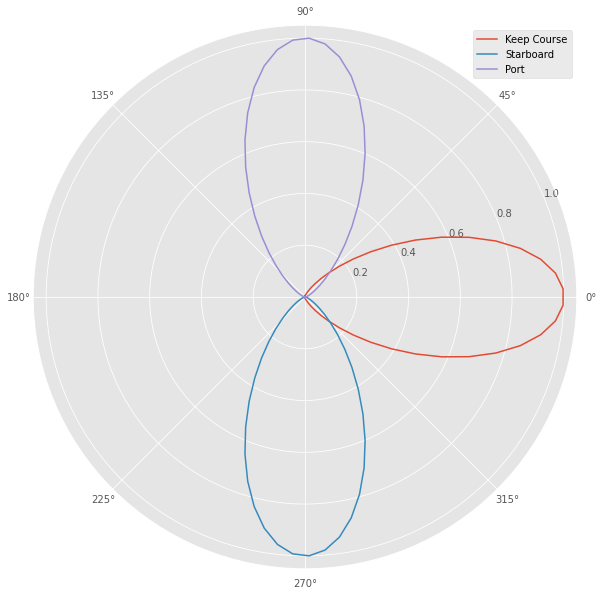
\includegraphics[width=0.7\textwidth]{figures/intention_angle.png}
    \caption{Normalized likelihood of different angles under different intention hypotheses. This is a polar plot where the angle represent $\theta_t^{(I=i)}$, the radius represent the probability. This is generated from \cref{eq:theta_intention_mixture} with $\mu_0=0$, $\mu_1 = -\frac{\pi}{2}$, $\mu_2=\frac{\pi}{2}$ and $\sigma_i=\frac{\pi}{8}$}
    \label{fig:intention_angle}
\end{figure}

\begin{figure}
    \centering
    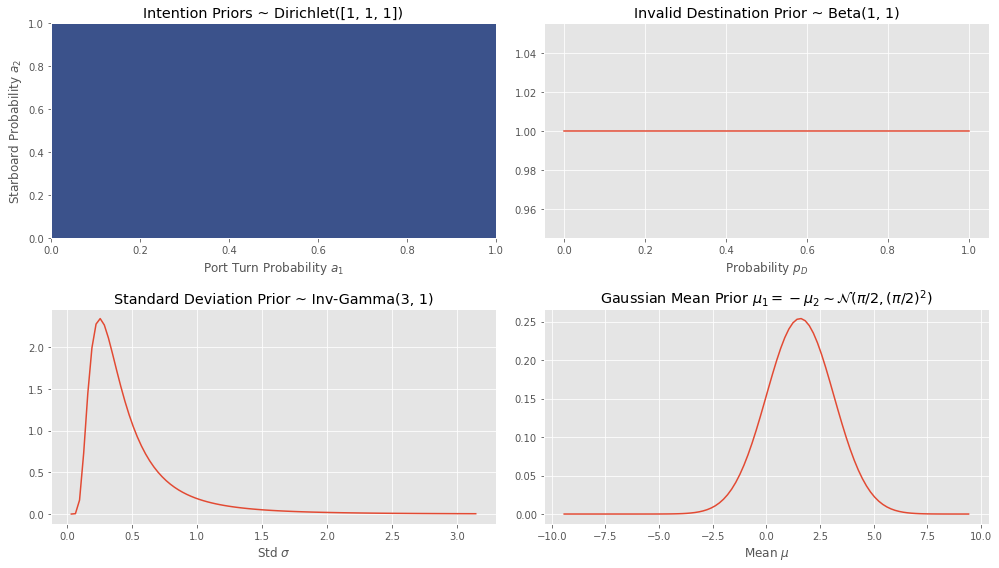
\includegraphics[width=1\textwidth]{figures/priors.png}
    \caption{Model priors for $\boldsymbol{\alpha}$, $p_D$, $\sigma$ and $\boldsymbol{\mu}$. The contour plot for $\boldsymbol{\alpha}$ shows $\alpha_1$ and $\alpha_2$, but $\alpha_0$ is implicitly included by the constraint $\alpha_0 = 1 - \alpha_1 - \alpha_2$. The priors for $\boldsymbol{\alpha}$ and $p_D$ are non-informative priors, while the priors for $\mu_2 = -\mu_1$ and $\sigma$ are informative priors selected by intuitive reasoning.}
    \label{fig:priors}
\end{figure}

The purpose of this chapter is to learn as much about the parameters $\boldsymbol{\alpha}$, $\mu$, $\sigma$ and $p_D$ from available observations $\mathcal{D}$, in this case only the angles $\mathcal{D} = \boldsymbol{\theta}$ are known. 

\section{Implementation}
Both \acrshort{mcmc} and \acrshort{vi} were implemented using Tensorflow Probability, as it has great support for both methods as well as it utilizes Tensorflows automatic differentiation to avoid dealing with error-prone calculations \cite{tensorflow2015-whitepaper}. The joint distribution in \cref{eq:example_joint} was implemented using the \texttt{JointDistributionSequential} distribution in TFP. (TODO: Add code in appendix)


\section{Dataset \& Benchmark}
The dataset was generated from $N=1000$ samples $\boldsymbol{\mathcal{D}}$ from \cref{eq:angle_complete_mixture} with fixed parameters. A successful inference should be able to regain the parameters $\boldsymbol{\alpha}$, $p_D$, $\mu_2 = -\mu_1$ and $\sigma$ from $\mathcal{D}$.

\section{Markov Chain Monte Carlo}
Hamiltonian Monte Carlo was implemented using Tensorflow Probability (TFP). The log posterior target density was then defined using \cref{eq:example_unnormalized_posterior} as 
\begin{align}\label{eq:example_ll}
\begin{split}
    ll &= \log \tilde{p}(\boldsymbol{\mu}, \sigma, p_D, \boldsymbol{\alpha})
\end{split}
\end{align}


The proposal distribution were transformed using the following transformations (Bijectors)

\begin{itemize}
\item Softmax \eqref{eq:softmax} to unconstrain sampling of $\{\boldsymbol{\alpha} \in (0, 1)^3\ | \sum x_i = 1\}$
\item Sigmoid \eqref{eq:sigmoid} to unconstrain sampling of $p_D \in (0, 1)$
\item Softplus \eqref{eq:softplus} to unconstrain sampling of $\sigma > 0$
\item Softplus \eqref{eq:softplus} to acheive unimodal sampling of $\mu > 0$
\end{itemize}

$20$ individual chains were randomly initialized by sampling from the prior. $30000$ samples were then drawn from each chain, were the first $10000$ samples are discarded due to burn-in. These values were selected by trial and error, and by inspecting the individual chains in order to confirm convergence.  

\section{Variational Inference}

\acrshort{vi} was implemented using an independent, transformed Gaussian distribution as surrogate density for each variable. Specifying this model was easily achieved by passing the following list of Bijectors to \texttt{tfp.experimental.vi.build\_factored\_surrogate\_posterior}.
\begin{itemize}
\item Softmax \eqref{eq:softmax} to transform $\mathcal{R}$ to $\{\boldsymbol{\alpha} \in (0, 1)^3\ | \sum x_i = 1\}$
\item Sigmoid \eqref{eq:sigmoid} to transform $\mathcal{R}$ to $p_D \in (0, 1)$
\item Softplus \eqref{eq:softplus} to transform $\mathcal{R}$ to $\sigma > 0$
\item Softplus \eqref{eq:softplus} to achieve unimodal distribution of $\mu \in \mathcal{R}$
\end{itemize}

The last Softplus Bijector is especially important for \acrshort{vi} and deserves further explanation. As the intention probabilities for $I=1$ and $I=2$ are symmetrical around $\theta=0$ and the Gaussian distribution offer support on the entire real line $\mathcal{R}$, the resulting marginal distribution for $\mu$ becomes bimodal. As the model is not identifiable from $\boldsymbol{\theta}$ alone, the data supports both modes. The prior do prioritize the positive values, but still offers support for negative values as well.  Using \acrshort{vi} with reverse \acrshort{kl} may therefore result in fitting the wrong mode, unless $\mu > 0$ is explicitly enforced by using a Softplus transformation to remove support for negative values. 

The Stochastic Gradient Descent (SGD) optimizer \texttt{tf.optimizers.Adam} was then used to optimize the reverse KL divergence by passing it to \texttt{tfp.vi.fit\_surrogate\_posterior} along with the same log posterior density used for \acrshort{mcmc}, expressed in \cref{eq:example_ll} \cite{tensorflow2015-whitepaper}. 

\section{Results}
A dataset of $N=1000$ samples were used to observe how well \acrshort{vi} and \acrshort{mcmc} are able to learn from data. The true parameters used to generate the datasets are summarized in \cref{tbl:example_params}. The parameters were selected such that the priors are reasonable, while also making sure that the true parameters are different from the prior max and mean (to verify that the values are actually learned from data). 
\begin{table}[h]
\centering
\begin{tabular}{lllll}
\textbf{Variable:}   & $\boldsymbol{\alpha}$ & $p_D$ & $\mu$                  & $\sigma$         \\ \hline
\textbf{Value:} & $[0.5, 0.3, 0.2]$     & $0.3$ & $\frac{\pi}{3}$ & $0.6$ \\
\end{tabular}
\caption{True values used to generate the dataset for example case 1.}
\label{tbl:example_params}
\end{table}


The posterior distribution when using \acrshort{mcmc} is shown in \cref{fig:example_mcmc_posterior} and shows how it is able to infer the intention probabilities $\boldsymbol{\alpha}$ from data, with the MAP estimates being pretty much spot-on. The uncertainty for the different intentions are however rather high, as multiple combinations of parameter values are able to explain the data rather well. The probability of invalid destination $p_D$ is also successfully reconstructed from observations, with rather low uncertainty. However, it it unable to distinguish between the mean $\mu$ and the standard deviation $\sigma$, resulting in high uncertainty and incorrect MAP estimates. The sampling took over 8 minutes in total for this dataset. 

\cref{fig:example_vi_posterior} show the performance of \acrshort{vi} on the same dataset. The marginal intention probability distribution for $p(\boldsymbol{\alpha} | \mathcal{D})$ are surrounding the true values, but the MAP estimates are off with around $10\%$ and $5\%$ for $p(I=0)$ and $p(I=1)$ respectively. \acrshort{vi} also severely underestimate the true uncertainty. For the invalid destination probability, the results are however much better with very similar results as \acrshort{mcmc}. For the mean $\mu$ and standard deviation $\sigma$, the results are comparable to \acrshort{mcmc}, though with less uncertainty. However, considering the optimization only used 22 seconds on the same computer, these results are quite impressive when compared to \acrshort{mcmc}.

Another dataset with only $N=50$ samples was generated to see how the methods behave will low amounts of data. \cref{fig:example_mcmc_vi_low_N} show how \acrshort{vi} is a bit overconfident on the intention probabilities and underestimate the uncertainty when compared to \acrshort{mcmc}. The results are otherwise very similar as shown in \cref{fig:example_mcmc_low_N} and \cref{fig:example_vi_low_N} for \acrshort{mcmc} and \acrshort{vi} respectively. Both methods are able to express the high uncertainty due to the limited amount of data available. 

Other datasets created with different parameters were also tested, though the plots are not included. Other datasets showed very similar results, only varying a bit on which variables the methods were able to correctly estimate. Random variations when generating the dataset also affected the final results, where some realizations of the data performed well and other performed poorly even if the parameters remained constant. 

The number of burn-in samples were somewhat arbitrarily chosen. However, by inspecting the individual chains in \cref{fig:example_mcmc_trace}, the individual chains appear to have reached the same stationary distribution and $10000$ burn-in samples are assumed to be enough for this specific problem.

\begin{figure}[h]
    \centering
    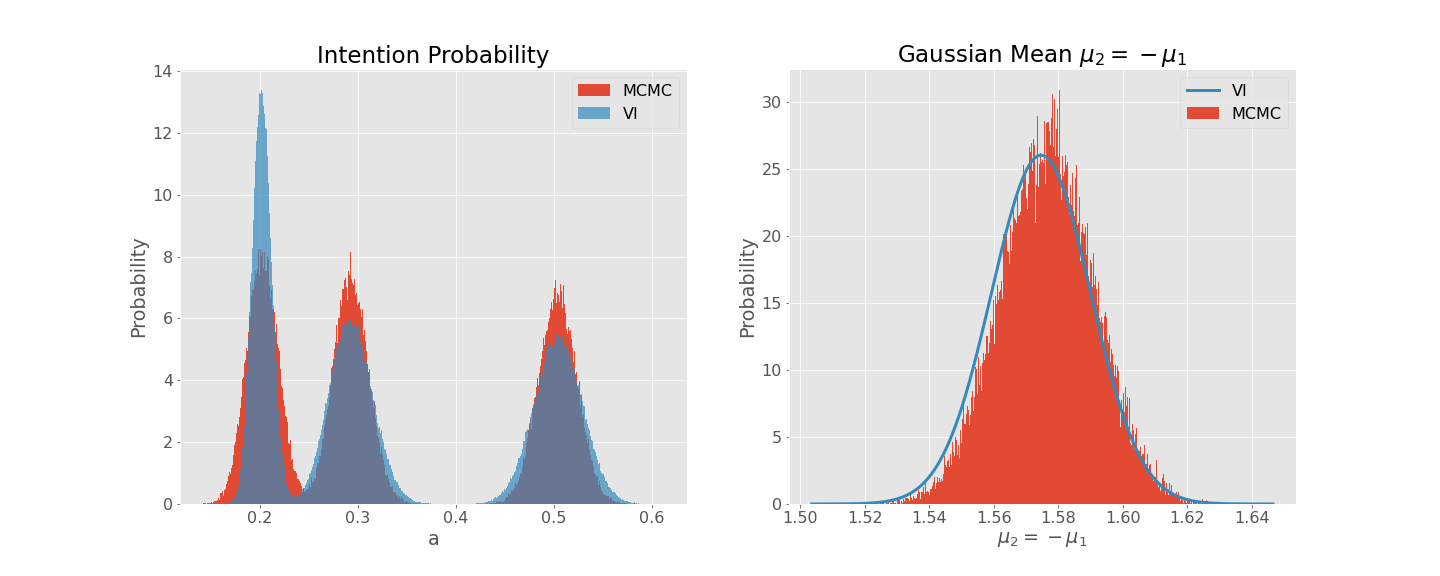
\includegraphics[width=\textwidth]{figures/example_vi_mcmc_comparison.png}
    \caption{The posterior distribution for intention probabilities and Gaussian mixture component means, found using MCMC and VI and plotted together to show how the methods give very comparable results. Note that all three intention probabilities are plotted together with the same color to highlight the differences between MCMC and VI. The plot shows how \acrshort{vi} underestimate the uncertainty when compared to \acrshort{mcmc}.}
    \label{fig:example_mcmc_vi_alphas}
\end{figure}

\begin{figure}[h]
    \centering
    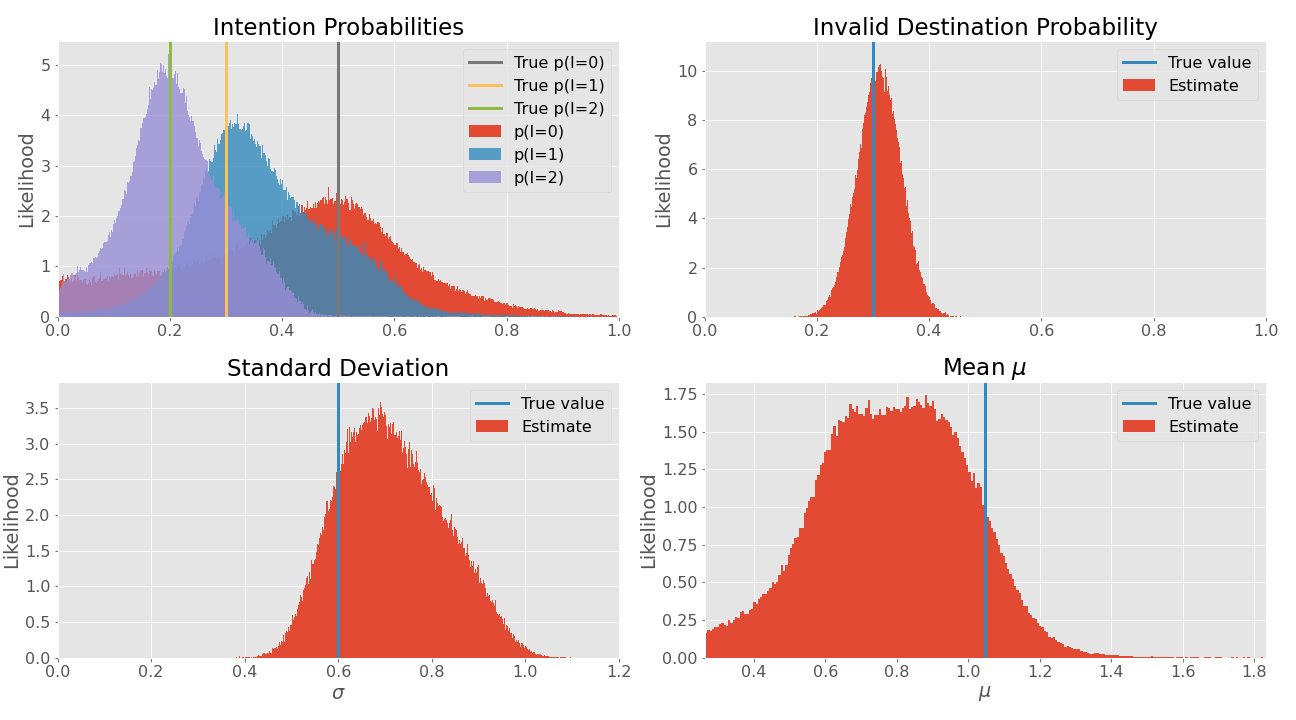
\includegraphics[width=\textwidth]{figures/example_mcmc.png}
    \caption{The posterior distribution for all variables using MCMC. The method is able to estimate the parameters from available data, though with rather high uncertainty. The MAP estimates are close to the true values for all parameters.}
    \label{fig:example_mcmc_posterior}
\end{figure}


\begin{figure}[h]
    \centering
    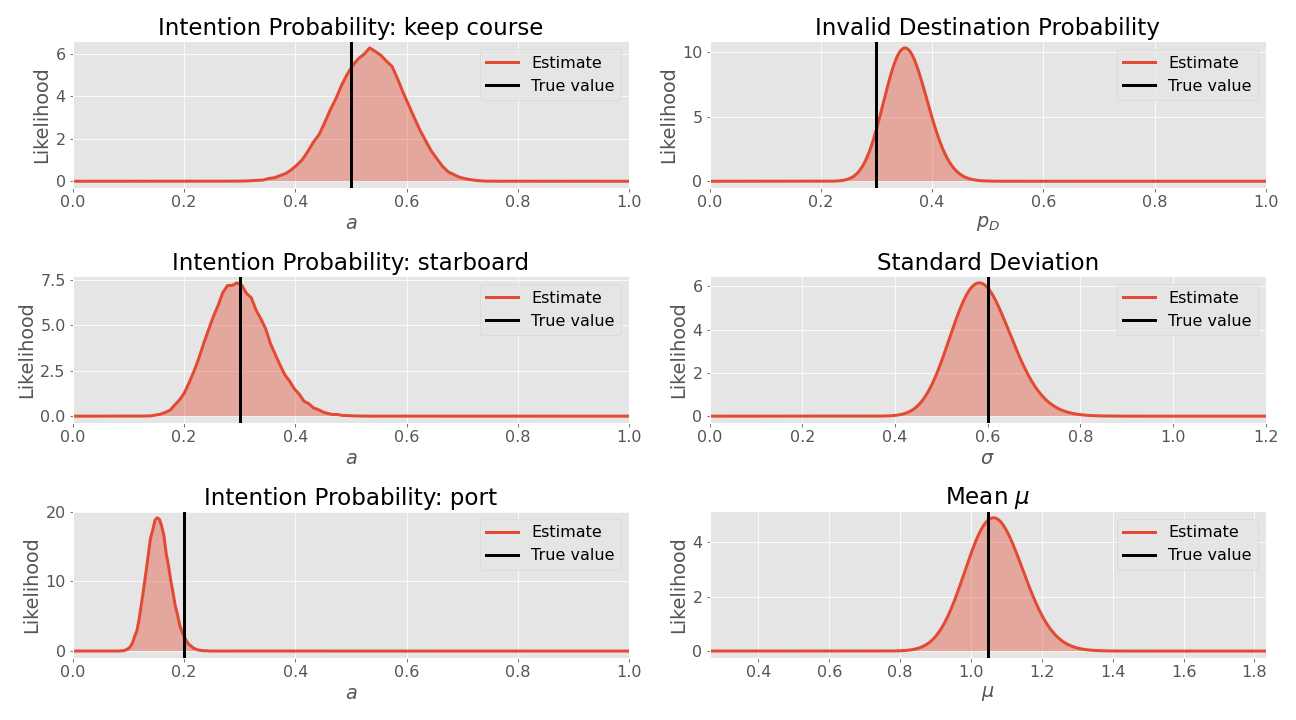
\includegraphics[width=\textwidth]{figures/example_vi.png}
    \caption{The posterior distribution for all variables using VI. The results are comparable to \acrshort{mcmc}, with very similar MAP estimates. The low uncertainty are however indicating overconfidence, especially when compared to \acrshort{mcmc}.}
    \label{fig:example_vi_posterior}
\end{figure}


\begin{figure}[h]
    \centering
    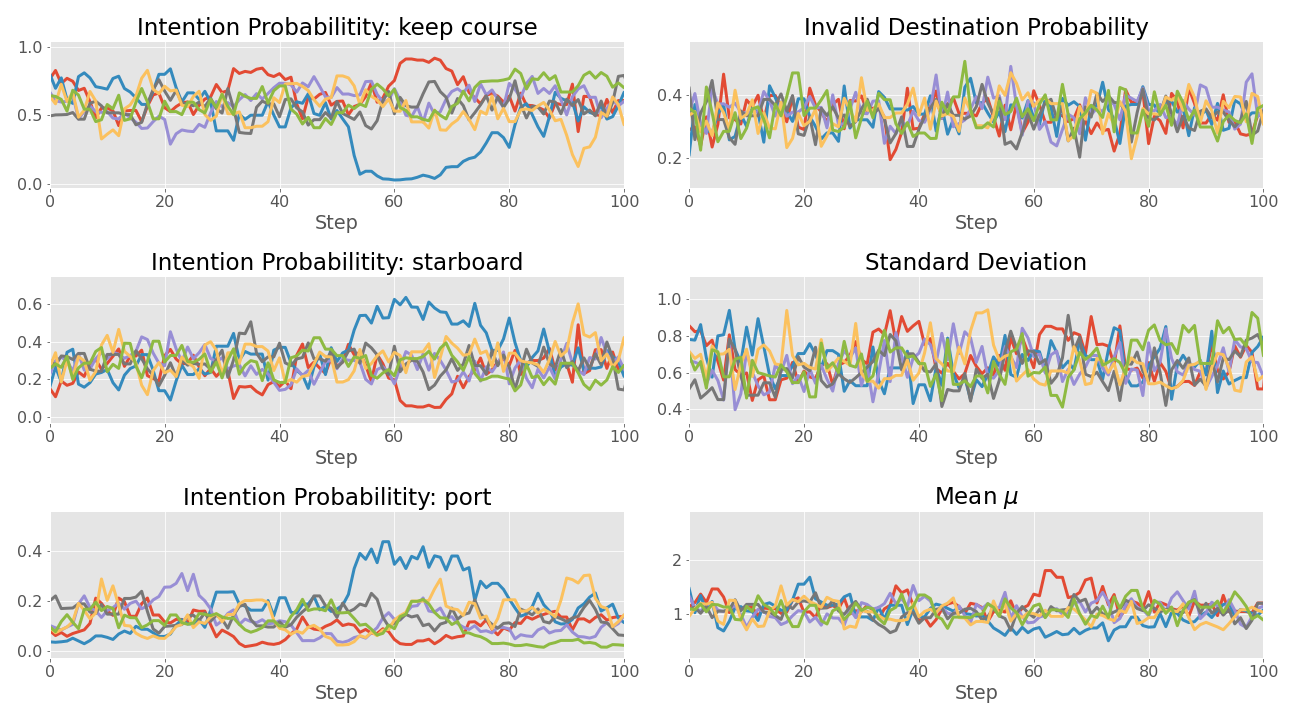
\includegraphics[width=\textwidth]{figures/example_mcmc_trace.png}
    \caption{Traceplot of the different chains. The chains appear to have reached a stationary distribution, and the current burn-in period of $5000$ samples are likely sufficient for this problem.}
    \label{fig:example_mcmc_trace}
\end{figure}

\begin{figure}[h]
    \centering
    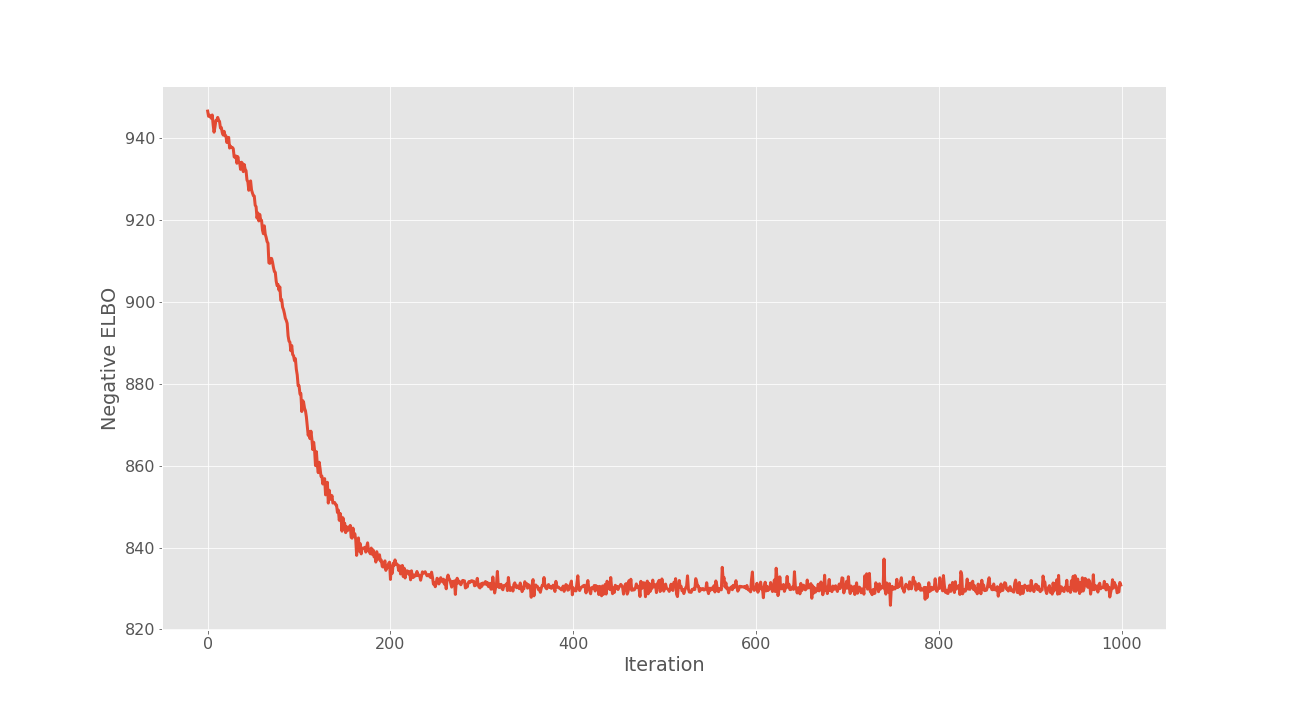
\includegraphics[width=\textwidth]{figures/example_vi_losses.png}
    \caption{Negative ELBO plotted against the fixed number of optimization steps for \acrshort{vi}. It reaches an optimum after less than $500$ steps and could in this case be stopped early to shorten the runtime.}
    \label{fig:example_vi_losses}
\end{figure}


\begin{figure}[h]
    \centering
    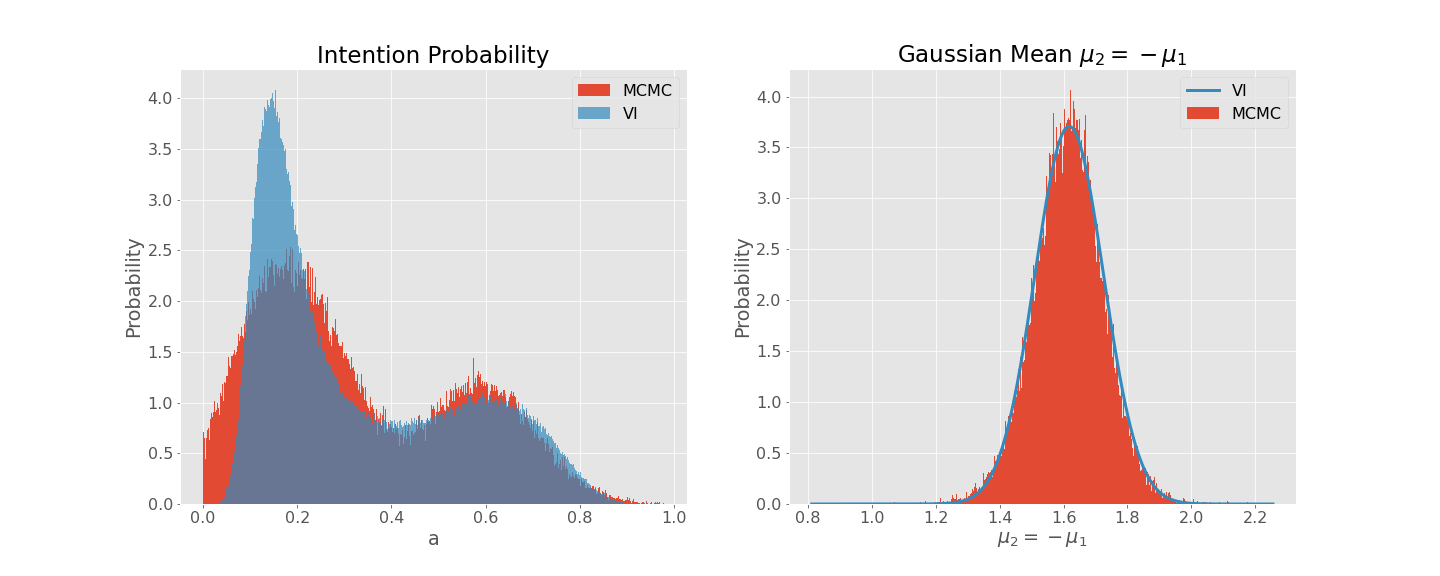
\includegraphics[width=\textwidth]{figures/example_vi_mcmc_comparison_low_N.png}
    \caption{Comparison of MCMC and VI for the parameters $\boldsymbol{\alpha}$ and $\mu$ with only $N=50$ samples. Both methods are able to express uncertainty due to low amount of data.}
    \label{fig:example_mcmc_vi_low_N}
\end{figure}

\begin{figure}[h]
    \centering
    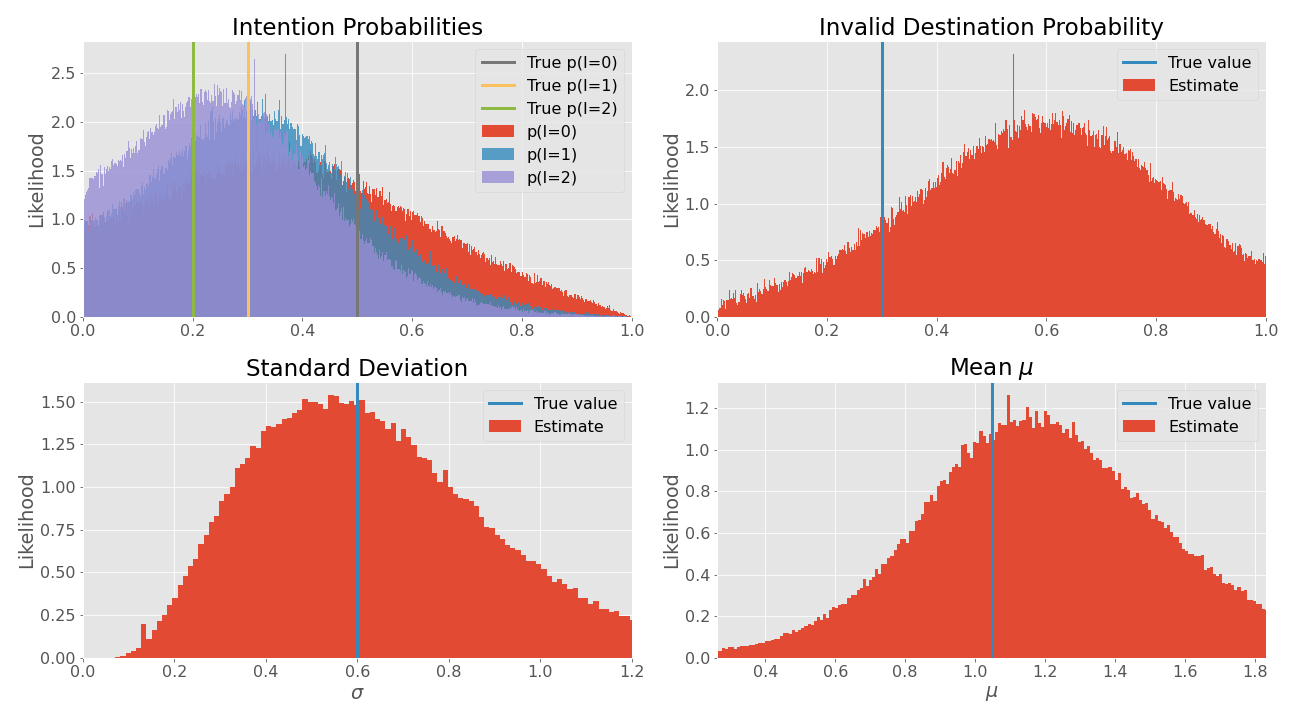
\includegraphics[width=\textwidth]{figures/example_mcmc_low_N.png}
    \caption{Posterior distribution approximated using \acrshort{mcmc} with only $N=50$ samples. The results shows large uncertainty for all parameters.}
    \label{fig:example_mcmc_low_N}
\end{figure}

\begin{figure}[h]
    \centering
    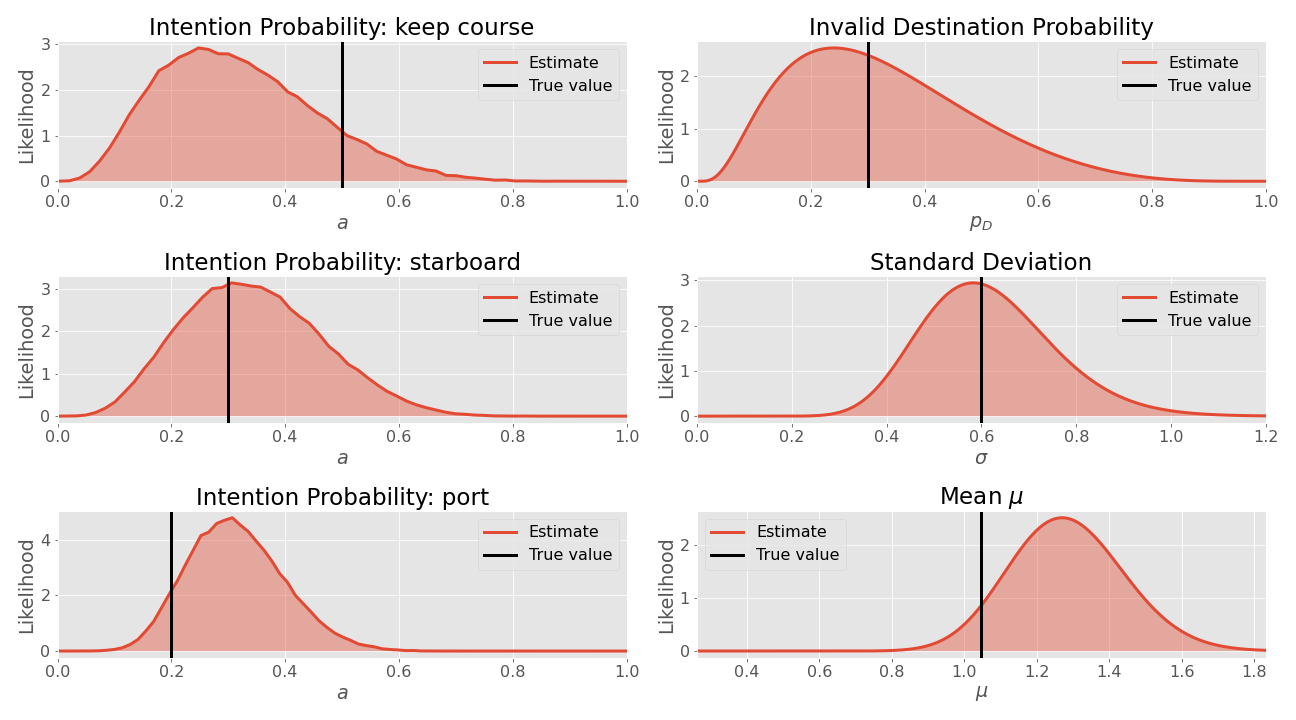
\includegraphics[width=\textwidth]{figures/example_vi_low_N.png}
    \caption{Posterior distribution approximated using \acrshort{vi} with only $N=50$ samples. The results shows large uncertainty for all parameters.}
    \label{fig:example_vi_low_N}
\end{figure}


